\begin{figure}[H]
\centering
\includegraphics[width=0.48\textwidth]{\FCNCFigures/tthML/showFake/faketau/prefit/NOMINAL/reg2l1tau1bnj_vetobtagwp70_highmet/tau_pt_0.pdf}
\includegraphics[width=0.48\textwidth]{\FCNCFigures/tthML/showFake/faketau/prefit/NOMINAL/reg2l1tau2bnj_vetobtagwp70_highmet/tau_pt_0.pdf}
\includegraphics[page=6,width=0.48\textwidth]{\FCNCFigures/tthML/showFake/faketau/prefit/NOMINAL/reg1l1tau2b2j_os_vetobtagwp70_highmet/tau_pt_0.pdf}
\includegraphics[page=6,width=0.48\textwidth]{\FCNCFigures/tthML/showFake/faketau/prefit/NOMINAL/reg1l1tau2b3j_os_vetobtagwp70_highmet/tau_pt_0.pdf}
\includegraphics[page=6,width=0.48\textwidth]{\FCNCFigures/tthML/showFake/faketau/prefit/NOMINAL/reg1l1tau2b2j_ss_vetobtagwp70_highmet/tau_pt_0.pdf}
\includegraphics[page=6,width=0.48\textwidth]{\FCNCFigures/tthML/showFake/faketau/prefit/NOMINAL/reg1l1tau2b3j_ss_vetobtagwp70_highmet/tau_pt_0.pdf}
\caption{各$t\bar{t}$控制区中$\tauhad$的$\pt$谱,图中将Fake tau的来源进行分类,其中的Fake tau本底包含所有的样本。可以看出其中部分区域与信号区有相似的行为:OS区被高估,SS区被低估。}
\label{fig:wjet_pt_CR}
\end{figure}
